\documentclass{article}
\usepackage[utf8]{inputenc}
\usepackage[a4paper, margin=17mm]{geometry}
\usepackage[norsk]{babel}
\usepackage{amssymb}
\usepackage{amsmath}
\usepackage{amsthm}
\usepackage{scrextend}
\usepackage{hyperref}
\usepackage{multicol}
\usepackage{tikz}
\usepackage{array}
\usepackage{mdframed}
\usepackage[american]{circuitikz}
\usepackage[small]{titlesec}

\hypersetup{colorlinks=true, 
			linkcolor=blue, 
			filecolor=magneta,
			urlcolor=cyan,
            citecolor=black,
}

\setlength{\columnsep}{1cm}

\newtheorem{thm}{Teorem}\surroundwithmdframed{thm}

\theoremstyle{definition}
\newtheorem{exx}[thm]{\color{blue}Eksempel}
\newtheorem{defnx}[thm]{Definisjon}
\newtheorem{oppg}{}
\newtheorem{merkx}{Merk}
\newtheorem{kommentarx}{Kommentar}
\newtheorem{spmx}{Spørsmål}
\newtheorem{innercustomoppg}{}
\newenvironment{customoppg}[1]
    {\renewcommand\theinnercustomoppg{#1}\innercustomoppg}
    {\endinnercustomoppg}

\newenvironment{defn}
{\pushQED{\qed}\renewcommand{\qedsymbol}{$\triangle$}\defnx}
{\popQED\enddefnx}
\newenvironment{ex}
{\pushQED{\qed}\renewcommand{\qedsymbol}{$\triangle$}\exx}
{\popQED\endexx}
\newenvironment{merk}
{\pushQED{\qed}\renewcommand{\qedsymbol}{$\triangle$}\merkx}
{\popQED\endmerkx}
\newenvironment{spm}
{\pushQED{\qed}\renewcommand{\qedsymbol}{$\triangle$}\spmx}
{\popQED\endspmx}

\theoremstyle{remark}
\newtheorem*{bevis}{Bevis}

\DeclareMathOperator{\diff}{d}

\usetikzlibrary{patterns,decorations.pathmorphing}

\newcommand{\springfig}[6]{%
\begin{scope}[xshift=#6,
              spring/.style = {decorate,
                              decoration = {aspect         = 0.5, 
                                            segment length = #1,
                                            amplitude      = 2mm,
                                            coil}}]

\path (0,0)                            coordinate (g) 
      (0,-0.5cm)                       coordinate (topspring) 
      (0, #2)                          coordinate (bottomspring) 
      (bottomspring) ++(0,-.3cm)       coordinate (pt2)
                      +(0cm,-#3)       coordinate (pt3)
                      +(1.25cm,-#3)    coordinate (#5 pt3);

  \node [platform,
        anchor = south] at (g)  {};
  \draw [very thick]    (-0.5,0)         -- (0.5,0);
  \draw                (topspring)     -- (g)
                      (bottomspring)  -- (pt2.north);
  \draw [spring]       (bottomspring)  -- (topspring);
  \draw [fill=black] (pt3) circle (#3) 
                          node[inner sep = 0,
                                scale     = #4,
                                text      = white]{$m$};
  \node[below=1.5*#3] at (pt3) {#5};
  \end{scope}
}

\begin{document}

\begin{center}
    \large{\textbf{Andreordens lineære differensialligninger}}
    \\
    \normalsize{Magnus Christie Ørke}
\end{center}
\vspace{\baselineskip}

\begin{multicols*}{2}
I dette kapitlet skal vi løse andreordens lineære differensiallikninger. Først behandler vi ligningene som genuint andreordens ligninger, og ser på ulike løsningsteknikker. Så skal vi se at andreordens ligninger kan skrives om til systemer av førsteordens ligninger ved hjelp av et variabelskifte, og at de to måtene å behandle ligningene på er i overensstemmelse.

\begin{ex}
Vi har tidligere sett at ligningen
\begin{equation*}
    \ddot{y}(t) + y(t) = 0
\end{equation*}
har generell løsning $c_1 \sin(t) + c_2 \cos(t)$. Dersom vi også har gitt to initialbetingelser
\begin{equation*}
  y(0) = a \ \textnormal{ og } \ \dot{y}(0) = b
\end{equation*} kan vi bestemme konstantene $c_1$ og $c_2$, og vi får spesiell løsning
\begin{equation*}
  y(t) = b \sin(t) + a \cos(t).
\end{equation*}
\end{ex}


\section*{Modellering av fysiske systemer}
Differensialligninger er svært nyttige for å beskrive systemer som involverer bevegelse og endring. I fysikk er differensiallikninger en sentral del av teorien, og ofte kan fysiske lover formuleres som differensialligninger. Et eksempel på dette er Newton's andre lov, som sier at summen av kreftene på et legeme er lik legemets masse multiplisert med akselerasjonen til legemet.

For mange situasjoner, slik som turbulens og strømning i fluider, er ligningene som oppstår svært vanskelige å løse. Derfor brukes hovedsaklig numeriske metoder. Man kan likevel finne løsninger til ligningene for enkelte enkle systemer, og vi skal nå se på noen av disse.

\begin{ex} \label{ex:fjær}
  Under er en figur av et lodd med masse $m$ som henger i en fjær.
  \begin{center}
    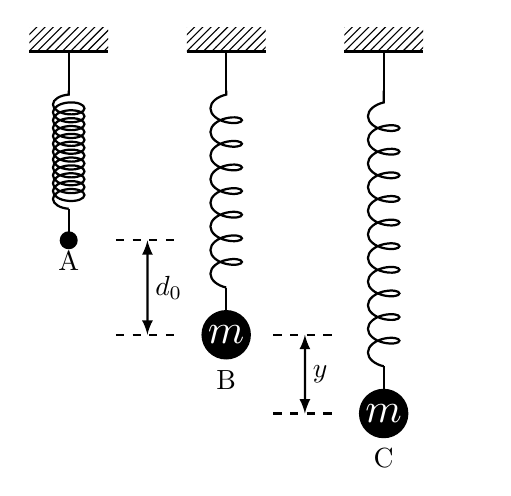
\begin{tikzpicture}[thick,
          every node/.style = {draw      = none,
                              inner sep = 0pt,
                              outer sep = 0pt},
          platform/.style   = {fill,
                              pattern = north east lines,
                              minimum width  = 1cm,
                              minimum height  =0.3cm}]
      \springfig{1mm}{-2cm}{0.1cm}{0}{A}{-2cm}
      \springfig{3mm}{-3cm}{0.3cm}{1.5}{B}{0cm}
      \springfig{3mm}{-4cm}{0.3cm}{1.5}{C}{2cm}

      \draw[dashed]
      (A pt3)  +(-0.4-0.25,0) -- coordinate (a1) +(0.4-0.25,0)
      (B pt3)  +(-0.4-0.25,0) -- coordinate (b1) +(0.4-0.25,0)
      (B pt3)  +(-0.4-2.25,0) -- coordinate (a2) +(0.4-2.25,0) 
      (C pt3)  +(-0.4-2.25,0) -- coordinate (b2) +(0.4-2.25,0);

      \draw[latex-latex] (a1) -- node[right=0.1cm]{$d_0$} (a2); 
      \draw[latex-latex] (b1) -- node[right=0.1cm]{$y$} (b2);
    \end{tikzpicture}  
  \end{center}
  I punkt A henger fjæren fritt uten lodd. I B har vi festet et lodd med masse $m$ til fjæren, og i C er det påført en kraft på loddet nedover, slik at fjæren strekkes en distanse $y$ fra likevektspunktet. Vi vet av erfaring at dersom vi nå slipper loddet vil det begynne å svinge om likevektspunktet, men hvordan skal vi beskrive dette matematisk?
  
  Ved å kombinere Newton's andre lov om kraft og akselerasjon med Hookes lov om fjærspenning får vi ligningen
  \begin{equation*}
    m \ddot{y}(t) + k y(t) = 0.
  \end{equation*}
  Dette er en andreordens differensialligning med konstante koeffisienter. Den ukjente er funksjonen $y(t)$ som beskriver loddets posisjon i forhold til likevekt avhengig av tid.
\end{ex}

\begin{ex} \label{ex:rc_parallell}
  Følgende figur viser en (RLC-) krets med en motstand, en spole og en kondensator koblet i parallell.
  \begin{center}
    \begin{circuitikz}
      \draw
      (0,0) node[ground] {}
      to[european resistor, l_ = $R$] (0,2)
      to[short] (2,2);
      \draw
      (2,0) node[ground] {}
      to[cute inductor, l_ = $L$] (2,2)
      to[short] (4,2);
      \draw
      (4,0) node[ground] {}
      to[capacitor, l = $C$] (4,2);
    \end{circuitikz}
  \end{center}
  Vi antar at kretsen har vært utsatt for en puls, og er interessert i hvordan spenningen $V(t)$ over kondensatoren varierer med tid. Vi kan kombinere Ohm's lov om spenningsfall over hver av komponentene med Kirchhoff's strømlov for å utlede følgene ligning for spenningen over kondensatoren.
  \begin{equation*}
    C \ddot{V}(t) + \frac{1}{R} \dot{V}(t) + \frac{1}{L} V(t) = 0.
  \end{equation*}
  Dette er et eksempel på en homogen differensialligning, siden høyresiden er null.
\end{ex}

\begin{ex} \label{ex:rlc_serie}
  Vi kan også koble motstanden, kondensatoren og spolen i serie. Denne gangen legger vi også inn en spenningskilde $V_s(t)$, slik som vist under.
  \begin{center}
    \begin{circuitikz}
      \draw
      (0,0)
      to[american voltage source, voltage dir=old, l={$V_s(t)$}, i^={$I(t)$}] (0,3)
      to[european resistor, l_ = $R$] (3,3)
      to[capacitor, l = $C$] (3,0)
      to[cute inductor, l_ = $L$] (0, 0);
    \end{circuitikz}
  \end{center}
  Kirchhoff's spenningslov kombinert med Ohm's lov for spenningsfall over komponentene gir oss nå at strømmen $I(t)$ gjennom kretsen vil være bestemt av
  \begin{equation*}
    L \ddot{I}(t) + R \dot{I}(t) + \frac{1}{C} I(t) = \dot{V}_s(t).
  \end{equation*}
  Merk at nå er høyresiden ikke lenger null, men en funksjon av tiden. Denne ligningen er derfor inhomogen.
\end{ex}


\section*{Andreordens ordinære differensialligninger}

En lineær andreordens ordinær differensialligning (ODE) er en ligning som kan skrives som
\begin{equation} \label{eq:generell_andreordens_ode}
  \ddot{y}(t) + p(t) \dot{y}(t) + q(t) y(t) = r(t),
\end{equation}
hvor $p(t)$, $q(t)$ og $r(t)$ er gitte funksjoner, og $y(t)$ er ukjent. Ligningen over har $1$ som koeffisient foran $\ddot{y}$, og alle andreordens lineære differensialligninger kan skrives om til denne formen ved å dele på koeffisienten foran $\ddot{y}$. Vi sier da at ligningen er på standard form.

Ligningen kalles ordinær når den ukjente funksjonen $y$ bare er avhengig av én variabel, i dette tilfelle $t$.

Dersom $r(t) = 0$ sier vi at ligningen er homogen. Vi skal også skille mellom ligninger med konstante koeffisienter, altså hvor $p(t)$ og $q(t)$ er konstanter, og ligninger hvor $p(t)$ og $q(t)$ er funksjoner av $t$.

Med et initialverdiproblem mener vi en andreordens lineær ODE sammen med to initialbetingelser
\begin{equation*}
    y(t_0) = a, \qquad \dot{y}(t_0) = b,
\end{equation*}
for den ukjente funksjonen $y(t)$.

Dersom funksjonen $y(t)$ er definert og to ganger kontinuerlig deriverbar på et åpent intervall $I$, og den i tillegg tilfredsstiller ligning \eqref{eq:generell_andreordens_ode}, sier vi at $y(t)$ er en løsning til \eqref{eq:generell_andreordens_ode}.

Man kan spørre seg hvorfor vi introduserer løsninger på åpne intervaller og ikke bare behandler ligningen på hele den reelle tallinjen. Det er mange grunner til dette, men hovedsaklig gir det oss mer fleksibilitet. Vi kan for eksempel tenke oss at vi vil løse en ligning som beskriver utviklingen av en størrelse som funksjon av tid, og det er da mer naturlig å lete etter en løsning på et positivt tidsintervall $(0, T)$ enn å jobbe med alle tidspunkter, også negative. Dette kommer likevel ikke til å spille en stor rolle i dette kapitlet.

Heretter skal vi betrakte løsningsteknikker for andreordens ODE-er med konstante koeffisienter. Vi kommer alltid til å anta at høyresiden $r(x)$ er en kontinuerlig funksjon.


\section*{Løsning av homogene ligninger}

Vi skal nå se på en standard metode for å løse ligningen
\begin{equation} \label{eq:homogen}
    \ddot{y}(t) + p \dot{y}(t) + q y(t) = 0,
\end{equation}
der $p$ og $q$ er to vilkårlige konstanter. Først gjør vi en observasjon om lineærkombinasjoner av løsninger til denne ligningen, og avklarer hva vi mener med en generell løsning.

\begin{thm} \label{thm:lin_komb_losning}
  Dersom to funksjoner $y_1(t)$ og $y_2(t)$ løser \eqref{eq:homogen}, er også alle lineærkombinasjoner av $y_1(t)$ og $y_2(t)$ en løsning til ligningen.
\end{thm}

\begin{bevis}
  Teoremet følger av at både ligningen, og operasjonen derivasjon, er lineære. La $\alpha y_1(t) + \beta y_2(t)$ være en lineærkombinasjon av løsningene, med $\alpha, \beta \in \mathbb{C}$. Da har vi
  \begin{equation*}
    \begin{split}
      & \frac{\mathrm{d}^2}{\mathrm{d} t^2}(\alpha y_1 + \beta y_2) + p \frac{\mathrm{d}}{\mathrm{d} t} (\alpha y_1 + \beta y_2) + q (\alpha y_1 + \beta y_2) \\
      & = \alpha (\ddot{y} + p \dot{y} + q y) + \beta (\ddot{y} + p \dot{y} + q y) = 0,
    \end{split}
  \end{equation*}
  hvor vi i siste steg har brukt antagelsen om at $y_1(t)$ og $y_2(t)$ er løsninger til ligningen. Dermed er $\alpha y_1(t) + \beta y_2(t)$ også en løsning.
\end{bevis}

\begin{defn}
    Med en generell løsning til ligning \eqref{eq:homogen} på et åpent intervall $I$ mener vi en funksjon på formen
    \begin{equation*}
      y_h(t) = c_1 y_1(t) + c_2 y_2(t),
    \end{equation*}
    hvor $c_1$ og $c_2$ er to ubestemte konstanter, og $y_1(t)$ og $y_2(t)$ er to lineært uavhengige funksjoner. Med en spesiell løsning til ligningen mener vi løsningen vi får ved å tilordne konstantene $c_1$ og $c_2$ i den generelle løsningen bestemte verdier gitt av initialbetingelser.
\end{defn}

Husk at to funksjoner er lineært uavhengige dersom $\alpha y_1(t) + \beta y_2(t) = 0$ impliserer at $y_1(y) = 0 = y_2(t)$, for alle $\alpha, \beta \in \mathbb{C}$. Hvis to lineært uavhengige funksjoner $y_1(t)$ og $y_2(t)$ begge løser \eqref{eq:homogen} sier vi at disse er en basis for løsningsrommet til ligningen.

Vi ønsker nå å finne en generell løsning til ligning \eqref{eq:homogen} for vilkårlige koeffisienter $p$ og $q$. Innsetting av funksjonen $y(t) = e^{\lambda t}$ som en løsningskandidat gir
\begin{equation*}
  (\lambda^2 + p \lambda + q) e^{\lambda t} = 0.
\end{equation*}
Dette betyr at dersom vi velger tallet $\lambda$ slik at
\begin{equation*}
  \lambda^2 + p \lambda + q = 0  
\end{equation*}
er ligningen oppfylt, og $e^{\lambda t}$ er en løsning. Vi kaller andregradsplynomet $\lambda^2 + p \lambda + q$ den karakteristiske ligningen til \eqref{eq:homogen}, og dersom vi tillater komplekse tall for $\lambda$ sier algebraens fundamentalteorem at vi alltid finne to røtter $\lambda_1$ og $\lambda_2$ for den karakteristiske ligningen. Disse gir dermed to løsninger
\begin{equation*}
  y_1(t) = e^{\lambda_1 t}\ \ \textnormal{ og }\ \ y_2(t) = e^{\lambda_2 t}.
\end{equation*}

Vi har nå tre kvalitativt ulike muligheter for hva den generelle løsningen er.

\paragraph*{To reelle røtter.} Dersom $p^2 - 4q > 0$ får vi to ulike reelle røtter $\lambda_1$ og $\lambda_2$. Da er den generelle løsningen til \eqref{eq:homogen} gitt ved
\begin{equation*}
  y_h(t) = c_1 e^{\lambda_1 t} + c_2 e^{\lambda_2 t},
\end{equation*}
fordi $e^{\lambda_1 t}$ og $e^{\lambda_2 t}$ er lineært uavhengige funksjoner for $\lambda_1 \neq \lambda_2$. Dette er det samme som å si at de to eksponensialfunksjonene utgjør en basis for løsningsrommet til ligningen.

\paragraph*{Én reell rot med dobbel multiplisitet.} Dersom $p^2 - 4q = 0$ vet vi at vi får en reell rot $\lambda$ med dobbel multiplisitet. Dette betyr at vi må lete etter en annen lineært uavhengig funksjon for å finne en generell løsning. Ved innsetting finner vi at funksjonen $te^{\lambda t}$ også er en løsning, og vi har dermed generell løsning
\begin{equation*}
  y_h(t) = (c_1 + c_2 t) e^{\lambda t}.
\end{equation*}

\paragraph*{To komplekse røtter.} Dersom vi har to komplekse røtter kan vi fortsatt skrive den generelle løsningen som
\begin{equation*}
  y_h(t) = c_1 e^{\lambda_1 t} + c_2 e^{\lambda_2 t},
\end{equation*}
men nå vil denne oppføre seg annerledes, og vi skal derfor også skrive den på en annen måte. Eulers formel gir oss at $e^{i t} = \cos(x) + i \sin(x)$. Vi observerer at røttene til den karakteristiske ligningen har samme reell del, og kan skrives på formen
\begin{equation*}
  \lambda_1 = r + i \omega \ \ \textnormal{ og }\ \ \lambda_2 = r - i \omega.
\end{equation*}
Vi kan altså skrive eksponensialfunksjonene $y_1(t)$ og $y_2(t)$ som
\begin{equation*}
  e^{rt} (\cos(\omega t) \pm i \sin(\omega t)).
\end{equation*}
Men ved Teorem \ref{thm:lin_komb_losning} er alle lineærkombinasjoner av $y_1(t)$ og $y_2(t)$ også løsninger til den homogene ligningen. På grunnlag av dette kan vi danne kombinasjonene 
\begin{equation*}
  \begin{split}
    & \frac{1}{2}y_1(t) + \frac{1}{2} y_2(t) = e^{r t} \cos(\omega t), \\
    & \frac{1}{2i}y_1(t) - \frac{1}{2i} y_2(t) = e^{r t} \sin(\omega t).
  \end{split}
\end{equation*}
Videre vet vi at disse funksjonene
lineært uavhengige. Den generelle løsningen for komplekse røtter $r \pm i \omega$ kan altså skrives på formen
\begin{equation*}
  y_h(t) = e^{r t} (c_1 \cos(\omega t) + c_2 \sin(\omega t)).
\end{equation*}

\begin{ex}
  Vi går tilbake til eksempel \ref{ex:fjær}. Posisjonen til loddet beskrives av
  \begin{equation*}
    m \ddot{y}(t) + ky(t) = 0.
  \end{equation*}
  Den karakteristiske ligningen er
  \begin{equation*}
    \lambda^2 + \frac{k}{m} = 0,
  \end{equation*}
  med røtter $\lambda = \pm i \sqrt{m / k}$. Den generelle løsningen er dermed gitt ved
  \begin{equation*}
    y(t) = c_1 \cos\bigg(\sqrt{\frac{k}{m}} t\bigg) + c_2 \sin\bigg(\sqrt{\frac{k}{m}} t\bigg),
  \end{equation*}
  hvor $c_1$ og $c_2$ er konstanter som kan bestemmes ved hjelp av initialbetingelser.
\end{ex}

\begin{ex}
  Vi kan legge til en friksjonskraft $F_f$ i fjærsystemet over. Dersom friksjonskraften er proporsjonal med hastigheten til loddet kan vi skrive $F_f = \gamma \dot{y}(t)$, hvor $\gamma$ er en friksjonskoeffisient. Ligningen for bevegelsen til loddet blir nå
  \begin{equation*}
    m \ddot{y}(t) + \gamma \dot{y}(t) + ky(t) = 0.
  \end{equation*}
  Begynn med å anta at $\gamma$ er liten i forhold til $m$ og $k$, og prøv nå å beskrive hvordan oppførselen til systemet endrer seg med økende friksjon.
\end{ex}

\begin{ex}
  Ligningen
  \begin{equation*}
    \ddot{y}(t) - y(t) = 0
  \end{equation*}
  har generell løsning
  \begin{equation*}
    y_h(t) = c_1 e^{t} + c_2 e^{-t}.
  \end{equation*}
\end{ex}

\begin{ex}
  Den generelle løsningen til
  \begin{equation*}
    \ddot{y}(t) - 2 \dot{y}(t) + y(t) = 0
  \end{equation*}
  er
  \begin{equation*}
    y_h(t) = (c_1 + c_2 t) e^t.
  \end{equation*}
\end{ex}

\begin{ex}
  Vi ser på RLC-kretsen fra eksempel \ref{ex:rc_parallell}. Den karakteristiske ligningen er
  \begin{equation*}
    \lambda^2 + \frac{1}{RC} \lambda + \frac{1}{LC} = 0,
  \end{equation*}
  med løsninger
  \begin{equation*}
    \lambda = - \frac{1}{2 R C} \pm \sqrt{\frac{1}{(2 R C)^2} - \frac{1}{LC}}.
  \end{equation*}
  Anta nå at vi har gitt verdiene $R = 50$ $\Omega$, $L = 20 $ mH og $C = 5$ $\mu$F, og at kretsen blir utsatt for en puls ved tiden $t = 0$ gitt ved $V(0) = 50$ V og $\dot{V}(0) = 0$. Da er $\lambda = -2000 \pm \sqrt{6 \cdot 10^6}$, og spenningen over kondensatoren er
  \begin{equation*}
    V(t) = 50 e^{- 2000 t} \cos(\sqrt{6 \cdot 10^6} t),
  \end{equation*}
  for $t > 0$.
\end{ex}

Et viktig spørsmål er om de generelle løsningene vi har funnet i eksemplene ovenfor er unike, eller om det også finnes andre løsninger. Vi har følgende teorem.

\begin{thm}
  Dersom funksjonen $y(t)$ løser den homogene ligningen \eqref{eq:homogen} på et åpent intervall $I$ med initialbetingelser
  \begin{equation*}
    y(t_0) = a, \qquad \dot{y}(t_0) = b
  \end{equation*}
  for $t_0 \in I$, er løsningen unik.
\end{thm}

Vi skal ikke bevise dette teoremet, men bruke det til å vise at vår betegnelse av en løsning på formen $c_1 y_1(t) + c_2 y_2(t)$ som en generell løsning til ligning \eqref{eq:homogen} er godt begrunnet.

\begin{thm} \label{thm:unik}
  Alle mulige løsninger til den homogene ligningen \eqref{eq:homogen} på et åpent intervall $I$ er på formen
  \begin{equation*}
    c_1 y_1(t) + c_2 y_2(t),
  \end{equation*}
  hvor $y_1(t)$ og $y_2(t)$ er en basis for løsningsrommet, og $c_1$ og $c_2$ er to konstanter.
\end{thm}

\begin{bevis}
  La $Y(x)$ være en vilkårlig løsning til \eqref{eq:homogen} på intervallet $I$. Med løsningsteknikken over kan vi alltid finne en generell løsning gitt ved
  \begin{equation*}
    y_h(x) = c_1 y_1(t) + c_2 y_2(t),
  \end{equation*}
  hvor $y_1(t)$ og $y_2(t)$ er lineært uavhengige. La nå $t_0$ være et vilkårlig punkt på intervallet $I$. Ligningssystemet
  \begin{equation*}
    \begin{bmatrix}
      y_1(t_0) & y_2(t_0) \\
      \dot{y}_1(t_0) & \dot{y}_2(t_0) \\
    \end{bmatrix}
    \begin{bmatrix}
      c_1 \\
      c_2 \\
    \end{bmatrix}
    =
    \begin{bmatrix}
      Y(t_0) \\
      \dot{Y}(t_0) \\
    \end{bmatrix}
  \end{equation*}
  har en unik løsning for $[c_1, c_2]^T$, siden determinanten $y_1 \dot{y}_2 - \dot{y}_1 y_2$ er ulik null. Dette følger igjen av at $y_1$ og $y_2$ er lineært uavhengige. Dermed kan vi finne koeffisienter $c_1$ og $c_2$ slik at 
  \begin{equation*}
    Y(t_0) = y_h(t_0), \qquad \dot{Y}(t_0) = \dot{y}_h(t_0).
  \end{equation*}
  På den annen side har vi ved Teorem \ref{thm:unik} at løsninger til initialverdiproblemet er unike. Dermed må $Y(t) = y_h(t)$ på hele $I$, og vi har vist at en vilkårlig løsning alltid kan skrives på formen til en generell løsning.
\end{bevis}


\section*{Løsning av inhomogene ligninger}
Vi skal nå se hvordan vi kan løse ligninger på formen
\begin{equation} \label{eq:inhomogen}
    \ddot{y}(t) + p \dot{y}(t) + q y(t) = r(t),
\end{equation}
hvor $p$ og $q$ er to vilkårlige konstanter, og $r(t)$ er en kontinuerlig funksjon. Når vi under refererer til den tilhørende homogene ligningen, mener vi ligning \eqref{eq:inhomogen} med $r(t)$ satt til null. Løsningene til den homogene ligningen spiller nemlig en rolle i også for den inhomogene ligningen, som beskrevet i følgende definisjon.

\begin{defn}
    Med en generell løsning til \eqref{eq:inhomogen} mener vi en løsning på formen
    \begin{equation*}
        y(t) = y_h(t) + y_p(t),    
    \end{equation*}
    hvor $y_h(t) = c_1 y_1(t) + c_2 y_2(t)$ er løsningen til den tilhørende homogene ligningen, og $y_p(t)$ er en partikulærløsning til den inhomogene ligningen som ikke inneholder ubestemte konstanter. Med en spesiell løsning mener vi løsningen vi får ved å tilordne konstantene $c_1$ og $c_2$ i $y_h(t)$ bestemte verdier i henhold til gitte initialbetingelser.
\end{defn}

Det finnes flere løsningstrategier for ligning \eqref{eq:inhomogen}. Ubestemte koeffisienters metode er praktisk i mange situasjoner og lett å forstå, men kan ikke brukes til alle typer funksjoner $r(t)$. Variasjon av parametre er en mer generell metode, men kan kreve litt mer regning. Vi skal se på begge.

\paragraph*{Ubestemte koeffisienters metode.} Metoden går ut på å gjette hva den partikulærløsningen til ligningen kan være avhengig av formen på $r(t)$. Først løser vi den homogene ligningen, før vi prøver å bestemme $y_p(t)$ ved å tilpasse parametre i en passende gjetningsfunksjon. For å illustrere dette ser vi på et eksempel.

\begin{ex}
  Betrakt ligningen
  \begin{equation*}
    \ddot{y}(t) + 3 \dot{y}(t) + 2 y(t) = 30 e^{2 t}.
  \end{equation*}
  Vi vet hvordan vi skal løse den homogene ligningen, og finner
  \begin{equation*}
    y_h(t) = c_1 e^{-t} + c_2 e^{-2 t}.
  \end{equation*}
  La oss nå anta at $y_p(t)$ er på formen $A e^{2t}$, for en ubestemt parameter $A$. Ved innsetting får vi da at
  \begin{equation*}
    (4 A + 6 A + 2 A) e^{2 t} = 30 e^{2 t},
  \end{equation*}
  og dermed må vi ha $A = 5/2$. Partikulærløsningen er altså $\frac{5}{2} e^{2 t}$, og den generelle løsningen er
  \begin{equation*}
    y(t) = c_1 e^{-t} + c_2 e^{-2 t} + \frac{5}{2} e^{2 t}.
  \end{equation*}
\end{ex}

I eksempelet over brukte vi kunnskapen om at eksponensialfunksjonen ikke endres mye under derivasjon. For å kunne gjette seg frem til riktig form på partikulærløsningen ut fra hvordan $r(t)$ ser ut kreves det erfaring. Likevel, siden metoden er mye brukt er det andre som har prøvd og feilet tidligere, og gode forslag til gjetninger kan oppsummeres som følger. Dersom $r(t)$ er gitt som en av funksjonene på venstre side i tabellen, bruker vi funksjonen til høyre, og tilpasser parametrene slik at ligningen blir oppfylt.

\begin{center}
  \begin{tabular}{m{0.15\textwidth} | m{0.25\textwidth}}
    $r(t)$ & $y_p(t)$ \\
    \hline \\
    $ke^{\lambda t}$ & $A e^{\lambda t}$ \\
    $k x^{n}$ & $A_n x^n + \cdots + A_0$ \\
    $k \cos(\omega t)$, $k \sin(\omega t)$ & \noindent\parbox[b]{\hsize}{$A \cos(\omega t) + B\sin(\omega t)$} \\
    $k e^{\lambda t} \cos(\omega t)$, $k e^{\lambda t} \sin(\omega t)$ & $e^{\lambda t} (A \cos(\omega t) + B\sin(\omega t))$ \\
  \end{tabular}
\end{center}

\begin{ex}
  Den homogene løsningen til
  \begin{equation*}
    \ddot{y}(t) + 9 y(t) = 6t^2
  \end{equation*}
  er
  \begin{equation*}
    y_h(t) = c_1 \cos(3t) + c_2 \sin(3t).
  \end{equation*}
  Dersom $y_p(t)$ er på formen $a_2 t^2 + a_1 t + a_0$ må koeffisientene tilfredsstille
  \begin{equation*}
    2a_2 + 9a_2 t^2 + 9a_1 t + 9 a_0 = 6 t^2,
  \end{equation*}
  og dermed har vi at $a_2 = 2/3$, $a_1 = 0$ og $a_0 = - 4/27$. Partikulærløsningen er
  \begin{equation*}
    y_p(t) = \frac{2}{3} t^2 - \frac{4}{27},
  \end{equation*}
  og den generelle løsningen er $y(t) = y_h(t) + y_p(t)$.
\end{ex}

\begin{ex}
  Ligningen for strømmen gjennom RLC-kretsen fra eksempel \ref{ex:rlc_serie} er
  \begin{equation*}
    L \ddot{I}(t) + R \dot{I}(t) + \frac{1}{C} I(t) = \dot{V}_s(t).
  \end{equation*}
  Det er naturlig å tenke seg at spenningskilden er på formen $V_s(t) = V_0 \sin(\omega t)$. Vi vet at den homogene løsningen er gitt ved å finne røttene til den karakteristiske ligningen
  \begin{equation*}
    \lambda^2 + \frac{R}{L} \lambda + \frac{1}{CL} = 0,
  \end{equation*}
  og vi har 
  \begin{equation*}
    \lambda = -\frac{R}{2L} \pm \sqrt{\left(\frac{R}{2L}\right)^2 - \frac{1}{CL}}.  
  \end{equation*}
  Siden $\dot{V}_s(t) = \omega V_0 \cos(\omega t)$ antar vi at partikulærløsningen er på formen $A \cos(\omega t) + B\sin(\omega t)$. Ved innsetting får vi da de to ligningene
  \begin{equation*}
    \begin{split}
      & - \omega^2 L A + \omega R B + \frac{1}{C} A = \omega V_0, \\
      & - \omega^2 L B - \omega R A + \frac{1}{C} B = 0.
    \end{split}
  \end{equation*}
  Vi innfører variabelen
  \begin{equation*}
    X = \omega L - \frac{1}{\omega C}.
  \end{equation*}
  Denne størrelsen er ofte kalt reaktansen til kretsen. De to ligningene blir da
  \begin{equation*}
    \begin{split}
      & BR - AX = V_0, \\
      & AR + BX = 0,
    \end{split}
  \end{equation*}
  og vi finner løsningen
  \begin{equation*}
    A = -\frac{V_0 X}{R^2 + X^2}, \qquad B = \frac{V_0 R}{R^2 + X^2}.
  \end{equation*}
  Med dette har vi altså bestemt både den homogene og den inhomogene løsningen til ligningen, og dermed strømmen $I(t)$.
\end{ex}

Til slutt nevner vi et triks. Hvis gjetningsfunksjonen vår for $y_p(t)$ også viser seg å være en homogen løsning til ligningen kan det være lurt å multiplisere gjetningsfunksjonen med $t$, slik som vi gjorde for røtter med dobbel multiplisitet for den homogene ligningen.

\paragraph*{Variasjon av parametre.} Ubestemte koeffisienters metode er begrenset til ligninger der funksjonen $r(t)$ og dens deriverte er relativt like. Dette fungerer godt for eksponensialfunksjonen, trigonometriske funksjoner og polynomer, men disse utgjør kun en liten klasse av alle mulige funksjoner. Vi ser på et motiverende eksempel.

\begin{ex} \label{ex:motiverende_eks}
  Betrakt ligningen
  \begin{equation*}
    \ddot{y}(t) + y(t) = \frac{1}{\cos(t)}.
  \end{equation*}
  Ved å se på de deriverte til $1 / \cos(t)$ blir det fort klart at vi ikke kan løse denne ligningen med ubestemte koeffisienters metode.
\end{ex}

Variasjon av parametre er en generell metode, og kan brukes for alle $r(t)$ som er kontinuerlige. Vi antar at $y_h(t) = c_1 y_1(t) + c_2 y_2(t)$ er den homogene løsningen til \eqref{eq:inhomogen}, og prøver å finne en partikulærløsning på formen
\begin{equation*}
  y_p(t) = v_1(t) y_1(t) + v_2(t) y_2(t),
\end{equation*}
hvor $v_1(t)$ og $v_2(t)$ er to ukjente funksjoner som må bestemmes. Funksjonen $y_p(t)$ må naturligvis tilfredsstille den inhomogene ligningen, og siden vi har to ukjente kan vi også anta at
\begin{equation*}
  \dot{v}_1(t) y_1(t) + \dot{v}_2(t) y_2(t) = 0.
\end{equation*}
Ved innsetting i \eqref{eq:inhomogen} får vi da at
\begin{equation*}
  \begin{split}
    r(t) & = v_1 (\ddot{y}_1 + p \dot{y}_1 + q y_1) + v_2 (\ddot{y}_1 + p \dot{y}_1 + q y_1) \\
    & + \dot{v}_1 \dot{y}_1 + \dot{v}_2 \dot{y}_2.
  \end{split}
\end{equation*}
De to første leddene er null som følge av at $y_1(t)$ og $y_2(t)$ er løsninger til den homogene ligningen. Sammen med antagelsen over gir dette det lineære ligningssystemet
\begin{equation*}
  \begin{bmatrix}
    y_1 & y_2 \\
    \dot{y}_1 & \dot{y}_2 \\
  \end{bmatrix}
  \begin{bmatrix}
    \dot{v}_1 \\
    \dot{v}_2 \\
  \end{bmatrix}
  =
  \begin{bmatrix}
    0 \\
    r(t) \\
  \end{bmatrix}
\end{equation*}
for $\dot{v}_1(t)$ og $\dot{v}_2(t)$. For å gjøre notasjonen enklere lar vi $W$ være determinanten til matrisen på venstre side av ligningen over. Siden $y_1(t)$ og $y_2(t)$ er lineært uavhengige er $W = y_1 \dot{y}_2 - \dot{y}_1 y_2 \neq 0$, og systemet har løsning
\begin{equation*}
  \dot{v}_1(t) = -\frac{y_2(t) r(t)}{W(t)}, \ \ \dot{v}_2(t) = \frac{y_1(t) r(t)}{W(t)}.
\end{equation*}
Dermed har vi at
\begin{equation*}
  v_1(t) = -\int \frac{y_2(t) r(t)}{W(t)} \mathop{dt}, \ \ v_2(t) = \int \frac{y_1(t) r(t)}{W(t)} \mathop{dt},
\end{equation*}
og partikulærløsningen er følgelig gitt ved
\begin{equation*}
  y_p(t) = v_1(t) y_1(t) + v_2(t) y_2(t).
\end{equation*}
Merk at integrasjonskonstantene i både $v_1(t)$ og $v_2(t)$ kan settes lik null, siden vi bare trenger én inhomogen løsning for å ha en generell løsning. Dette vil bli videre begrunnet av Teorem \ref{thm:alle_mulige_losn_inhomogen}.

\begin{ex}
  Vi løser ligningen fra eksempel \ref{ex:motiverende_eks}. Denne har homogen løsning
  \begin{equation*}
    y_h(t) = c_1 \cos(t) + c_2 \sin(t)
  \end{equation*}
  for to konstanter $c_1$ og $c_2$. Videre har vi at
  \begin{equation*}
    W(t) = \cos^2(t) + \sin^2(t) = 1
  \end{equation*}
  og dermed
  \begin{equation*}
    \begin{split}
      & v_1(t) = \int \frac{\sin(t)}{\cos(t)} \mathop{dt} = \ln(\cos(t)), \\
      & v_2(t) = \int 1 \mathop{dt} = t.
    \end{split}
  \end{equation*}
  Partikulærløsningen til ligningen er altså
  \begin{equation*}
    y_p(t) = \ln(\cos(t)) \cos(t) + t \sin(t),
  \end{equation*}
  og den generelle løsningen er $y(t) = y_h(t) + y_p(t)$.
\end{ex}

\begin{ex}
  Ligningen
  \begin{equation*}
    \ddot{y}(t) - 2\dot{y}(t) + y(t) = \frac{e^t}{t^2 + 1}
  \end{equation*}
  har homogen løsning
  \begin{equation*}
    y_h(t) = c_1 e^t + c_2 t e^{t}.
  \end{equation*}
  Nå kan vi regne ut at $W(t) = e^{2t}$, og dermed
  \begin{equation*}
    \begin{split}
      & v_1(t) = - \int \frac{t e^t e^t}{(t^2 + 1) e^2t} \mathop{dt} = - \ln(t^2 + 1), \\
      & v_2(t) = - \int \frac{e^t e^t}{(t^2 + 1) e^2t} \mathop{dt} = \arctan(t).
    \end{split}
  \end{equation*}
  Partikulærløsningen er altså
  \begin{equation*}
    y_p(t) = - e^t \ln(t^2 + 1) + t e^t \arctan(t).
  \end{equation*}
\end{ex}

Også for inhomogene ligninger beskriver den generelle løsningen $y_h(t) + y_p(t)$ alle mulige løsninger. Vi formulerer dette som et teorem, men inkluderer ikke beviset.

\begin{thm} \label{thm:alle_mulige_losn_inhomogen}
  Alle mulige løsninger til \eqref{eq:inhomogen} kan skrives ved å tilordne bestemte verdier til konstantene $c_1$ og $c_2$ i den generelle løsningen $y(t) = y_h(t) + y_p(t)$ til ligningen.
\end{thm}


\section*{Omformulering til systemer av førsteordens ligninger}
Selv om vi tilsynelatende har jobbet med andreordens differensialligninger i dette kapitlet har teorien en ekvivalent formulering som systemer av førsteordens ligninger. Ved å innføre de nye variablene
\begin{equation*}
  v_1(t) = y(t)\ \ \textnormal{ og }\ \ v_2(t) = \dot{y}(t)
\end{equation*}
kan vi omformulere ligning \eqref{eq:inhomogen} til systemet
\begin{equation*}
  \begin{bmatrix}
    \dot{v}_1 \\
    \dot{v}_2 \\
  \end{bmatrix}
  =
  \begin{bmatrix}
    0 & 1 \\
    -p & -q \\
  \end{bmatrix}
  \begin{bmatrix}
    v_1 \\
    v_2 \\
  \end{bmatrix}
  +
  \begin{bmatrix}
    0 \\
    r(t) \\
  \end{bmatrix}.
\end{equation*}
Dersom i tillegg $r(t) = 0$ og ligningen er homogen har vi det homogene systemet
\begin{equation*}
  \begin{bmatrix}
    \dot{v}_1 \\
    \dot{v}_2 \\
  \end{bmatrix}
  =
  \begin{bmatrix}
    0 & 1 \\
    -p & -q \\
  \end{bmatrix}
  \begin{bmatrix}
    v_1 \\
    v_2 \\
  \end{bmatrix}.
\end{equation*}
Slike systemer har vi lært å løse tidligere ved hjelp av den karakteristiske ligningen man får ved å finne egenverdiene til matrisen
\begin{equation*}
  \begin{bmatrix}
    0 & 1 \\
    -p & -q \\
  \end{bmatrix}.
\end{equation*}
Nå er det ikke vanskelig å se at det å finne en løsning for $[v_1, v_2]^{T}$ er helt tilsvarende det å finne $y(t)$ slik vi gjorde ovenfor, og at metodene gir samme resultat. Dette gjelder selvfølgelig også for den inhomogene ligningen.

\newpage

\section*{Oppgaver \footnote{Flere av oppgavene er hentet fra Tom Lindstrøm: \textit{Kalkulus}. (2006, 3. utgave).}}

\begin{oppg}
  Finn den generelle løsningen til ligningene
  \begin{multicols*}{2}
    \begin{itemize}
      \item[(a)] $\ddot{y} + \dot{y} - 6 y = 0$
      \item[(b)] $\ddot{y} + 5\dot{y} + 4y = 0$
      \item[(c)] $\ddot{y} + 6\dot{y} + 9y = 0$
      \item[(d)] $\ddot{y} - 2\dot{y} + 5y = 0$
      \item[(e)] $\ddot{y} + 2\dot{y} + 7y = 0$
      \item[(f)] $4\ddot{y} - 4\dot{y} + y = 0$  
    \end{itemize}
  \end{multicols*}
\end{oppg}

\begin{oppg}
  Finn løsningen til initialverdiproblemene
  \begin{itemize}
    \item[(a)] $\ddot{y} - 5\dot{y} + 4y = 0, \qquad y(0) = 2,\ \ \dot{y}(0) = -4$
    \item[(b)] $\ddot{y} - \dot{y} + \frac{y}{2} = 0, \qquad y(0) = 0,\ \ \dot{y}(0) = 7$
    \item[(c)] $\ddot{y} - 4\dot{y} - y = 0, \qquad y(1) = 2,\ \ \dot{y}(1) = -1$
    \item[(d)] $\ddot{y} + 4\dot{y} + 5y = 0, \qquad y(0) = 0,\ \ \dot{y}(0) = 1$
    \item[(e)] $\ddot{y} - 6\dot{y} + 9y = 0, \qquad y(1) = -e^3,\ \ \dot{y}(1) = -6e^3$
  \end{itemize}
\end{oppg}

\begin{oppg}  
  Betrakt ligningen
  \begin{equation*}
    \ddot{y} - \dot{y} - 2y = e^t
  \end{equation*}
  \begin{itemize}
    \item[(a)] Finn den generelle løsningen til den homogene ligningen.
    \item[(b)] Finn en partikulærløsning til ligningen.
    \item[(c)] Finn den spesielle løsningen til den inhomogene ligningen med initialbetingelser $y(0) = \dot{y}(0) = 2$.
  \end{itemize}
\end{oppg}

\begin{oppg}  
  Finn den generelle løsningen til ligningene
  \begin{itemize}
    \item[(a)] $\ddot{y} + 3\dot{y} + 2y = 30e^{2t}$
    \item[(b)] $\ddot{y} - 2\dot{y} - 8y = 6 - 8t$
    \item[(c)] $\ddot{y} + 2\dot{y} + 5y = \cos(t)$
    \item[(d)] $\ddot{y} - 8\dot{y} + 6y = t^2$
    \item[(e)] $\ddot{y} + 4\dot{y} + 4y = e^{-2t} \sin(2t)$
    \item[(f)] $\ddot{y} + 4\dot{y} + 5y = 25t^2 + 13\sin(2t)$ 
  \end{itemize}
\end{oppg}

\begin{oppg}  
  Betrakt ligningen
  \begin{equation*}
    \ddot{y} - 4\dot{y} + 4y = t^2 e^t
  \end{equation*}
  \begin{itemize}
    \item[(a)] Finn den generelle løsningen til den homogene ligningen.
    \item[(b)] Finn en partikulærløsning til ligningen.
    \item[(c)] Finn den spesielle løsningen til den inhomogene ligningen med initialbetingelser $y(0) = 0$ og $y'(0) = 2$.
  \end{itemize}
\end{oppg}

\begin{oppg}
  Er løsningene til følgende ligninger et vektorrom? Dersom svaret er ja, finn en basis for løsningsrommet.
  \begin{itemize}
    \item[(a)] $4\ddot{y} - 20\dot{y} + 25y = 0$
    \item[(b)] $\ddot{y} - 2y + 10 = 0$
    \item[(a)] $\ddot{y} + 9y = \cos(t) + \frac{1}{3} \cos(3t)$
    \item[(a)] $100\ddot{y} + 20\dot{y} = 99y$
    \item[(a)] $t \ddot{y} + y = 1$ 
  \end{itemize}
\end{oppg}

\begin{oppg}  
  Betrakt ligningen
  \begin{equation*}
    \ddot{y} - 12\dot{y} + 35y = 0.
  \end{equation*}
  \begin{itemize}
    \item[(a)] Finn den generelle løsningen til ligningen.
    \item[(b)] Skriv ligningen som et system av førsteordens differensialligninger på formen $\dot{\boldsymbol{y}}= A\boldsymbol{y}$. Finn egenverdiene til matrisen $A$, og bruk dette til å løse ligningen for $\boldsymbol{y}$.
  \end{itemize}
\end{oppg}

\begin{oppg}  
  Betrakt ligningen
  \begin{equation*}
    \ddot{y} + 2y = t^2.
  \end{equation*}
  \begin{itemize}
    \item[(a)] Finn den generelle løsningen til ligningen.
    \item[(b)] Skriv ligningen som et system av førsteordens differensialligninger på formen $\dot{\boldsymbol{y}}= A\boldsymbol{y} + \boldsymbol{\mathrm{f}}$. Finn egenverdiene til matrisen $A$, og bruk dette til å løse ligningen for $\boldsymbol{y}$.
  \end{itemize}
\end{oppg}

\begin{oppg}  
  Anta at to funksjoner $y_1(t)$ og $y_2(t)$ tilfredsstiller følgende system av differensialligninger
  \begin{equation*}
    \begin{split}
      & \dot{y}_1 = - y_1 - y_2, \qquad y_1(0) = 0\\
      & \dot{y}_2 = 5y_1 - 3y_2, \qquad y_2(0) = 2\\
    \end{split}
  \end{equation*}
  \begin{itemize}
    \item[(a)] Vis at $y_1(t)$ tilfredsstiller ligningen
    \begin{equation*}
      \ddot{y}_1 + 4\dot{y}_1 + 8y_1 = 0, \qquad y_1(0) = 0,\ \ \dot{y}_1(0) = -2.
    \end{equation*}
    \item[(b)] Finn $y_1(t)$.
    \item[(c)] Finn $y_2(t)$.
  \end{itemize}
\end{oppg}

\begin{oppg}  
  Betrakt følgende krets.
  \begin{center}
    \begin{circuitikz}
      \draw
      (0,0)
      to[american voltage source, voltage dir=old, l={$V_s(t)$}, i^={$I(t)$}] (0,3)
      to[european resistor, l_ = $R$] (3,3)
      to[capacitor, l = $C$] (3,0)
      to[short] (0, 0);
    \end{circuitikz}
  \end{center}
  \begin{itemize}
    \item[(a)] Utled en ligning for strømmen i kretsen som funksjon av tid.
    \item[(b)] Anta at $C=0.05\ \mathrm{F}$, $R=5\ \mathrm{\Omega}$ og $V_s=12\ \mathrm{V}$. Finn en generell løsning for strømmen i kretsen.
  \end{itemize}
\end{oppg}

\begin{oppg}  
  Betrakt følgende krets.
  \begin{center}
    \begin{circuitikz}
      \draw
      (0,0)
      to[american voltage source, voltage dir=old, l={$V_s(t)$}, i^={$I(t)$}] (0,3)
      to[european resistor, l_ = $R$] (3,3)
      to[short] (3,0)
      to[cute inductor, l_ = $L$] (0, 0);
    \end{circuitikz}
  \end{center}
  \begin{itemize}
    \item[(a)] Utled en ligning for strømmen i kretsen som funksjon av tid.
    \item[(a)] Anta at $V_s(t) = V_0 \sin(\omega t)$. Finn en generell løsning for strømmen for vilkårlige konstanter $R$, $L$, $V_0$ og $\omega$. 
  \end{itemize}
\end{oppg}

\begin{oppg}  
  La $N_1(t)$ og $N_2(t)$ være antallet individer av to dyrearter som en funksjon av tid. Vi introduserer to skalerte funksjoner
  \begin{equation*}
    \begin{split}
      & x(t) = N_1(t) - 300, \\
      & y(t) = N_2(t) - 10\ 000. \\
    \end{split}
  \end{equation*}
  Samspillet mellom de to artene kan modelleres av følgende system differensialligninger.
    \begin{equation*}
      \begin{split}
        & \dot{x}(t) = by(t), \\
        & \dot{y}(t) = -cx(t). \\
      \end{split}
    \end{equation*}
  \begin{itemize}
    \item[(a)] Hvilken art er rovdyr og hvilken er byttedyr?
    \item[(b)] Vis at $\ddot{x}(t) = -bc x(t)$.
    \item[(c)] Anta at $x(0) = x_0$ og $y(0) = y_0$. Finn $x(t)$ og $y(t)$.
    \item[(d)] Anta $b=0.05$, $c=84$ og $N_1(0) = 300$, $N_2(0) = 1400$. Plot antallet individer i de to populasjonene som en funksjon av tid.
  \end{itemize}
\end{oppg}



\newpage
\section*{Løsningsforslag}

\begin{customoppg}{1}
  Ved å regne ut røttene til det karakteristiske polynomet til ligningene finner man
  \begin{itemize}
    \item[(a)] $y(t) = c_1 e^{2t} + c_2 e^{-3t}$
    \item[(b)] $y(t) = c_1 e^{-4t} + c_2 e^{-t}$
    \item[(c)] $y(t) = c_1 e^{-3t} + c_2 te^{-3t}$
    \item[(d)] $y(t) = e^t (c_1 \cos(2t) + c_2 \sin(2t))$
    \item[(e)] $y(t) = e^{-t} (c_1 \cos(\sqrt{6}t) + c_2 \sin(\sqrt{6}t))$
    \item[(f)] $y(t) = c_1 e^{\frac{1}{2}t} + c_2 t e^{\frac{1}{2}t}$
  \end{itemize}
\end{customoppg}

\begin{customoppg}{2}
  \leavevmode
  \begin{itemize}
    \item[(a)] $y(t) = -2e^{4t} + 4e^t$
    \item[(b)] $y(t) = 14e^{\frac{t}{2}} \sin\big(\frac{t}{2}\big)$
    \item[(c)] $y(t) = \left( 1 - \frac{\sqrt{5}}{2} \right)e^{(2 + \sqrt{5})(t - 1)} + \left( 1 + \frac{\sqrt{5}}{2} \right)e^{(2 - \sqrt{5})(t - 1)}$
    \item[(d)] $y(t) = e^{-2t}\sin(t)$
    \item[(e)] $y(t) = 2e^{3t} - 3te^{3t}$
  \end{itemize}
\end{customoppg}  

\begin{customoppg}{3}
  \leavevmode
  \begin{itemize}
    \item[(a)] $y_h(t) = c_1e^{-t} + c_2e^{2t}$.
    \item[(b)] Ved å anta at $y_p(t) = Ae^t$ finner vi at
    \begin{equation*}
      (A - A - 2A) e^t = e^t.
    \end{equation*}
    Dermed er $y_p(t) = - \frac{1}{2} e^t$.
    \item[(c)] Den spesielle løsningen er gtt ved
    \begin{equation*}
      \frac{5}{6} e^{-t} + \frac{5}{3} e^{2t} - \frac{1}{2} e^t.
    \end{equation*} 
  \end{itemize}
\end{customoppg}

\begin{customoppg}{5}
  \leavevmode
  \begin{itemize}
    \item[(a)] $y_h(t) = c_1e^{2t} + c_2te^{2t}$.
    \item[(b)] Ved variasjon av parametre finner man at
    \begin{equation*}
      y_h(t) = t^2 e^t + 4te^t + 6e^t.
    \end{equation*}
    \item[(c)] $y(t) = t^2 e^t + 4te^t + 4te^{2t} - 6 e^{2t} + 6e^t$.
  \end{itemize}
  
\end{customoppg}



\end{multicols*}
\end{document}

Med denne formuleringen i bakhodet er det naturlig å tenke seg at man også kan løse høyere ordens lineære ordinære differensialligninger uten at teorien blir særlig mye vanskeligere. Det er nesten sant. Ved høyere ordens ligninger er man for eksempel nødt til å finne egenverdier til større matriser. Men det er verdt å ta med seg at løsingen av slike ligninger i stor grad dreier seg om lineær algebra.